\documentclass[twoside]{book}

% Packages required by doxygen
\usepackage{calc}
\usepackage{doxygen}
\usepackage{graphicx}
\usepackage[utf8]{inputenc}
\usepackage{makeidx}
\usepackage{multicol}
\usepackage{multirow}
\usepackage{textcomp}
\usepackage[table]{xcolor}

% Font selection
\usepackage[T1]{fontenc}
\usepackage{mathptmx}
\usepackage[scaled=.90]{helvet}
\usepackage{courier}
\usepackage{amssymb}
\usepackage{sectsty}
\renewcommand{\familydefault}{\sfdefault}
\allsectionsfont{%
  \fontseries{bc}\selectfont%
  \color{darkgray}%
}
\renewcommand{\DoxyLabelFont}{%
  \fontseries{bc}\selectfont%
  \color{darkgray}%
}

% Page & text layout
\usepackage{geometry}
\geometry{%
  a4paper,%
  top=2.5cm,%
  bottom=2.5cm,%
  left=2.5cm,%
  right=2.5cm%
}
\tolerance=750
\hfuzz=15pt
\hbadness=750
\setlength{\emergencystretch}{15pt}
\setlength{\parindent}{0cm}
\setlength{\parskip}{0.2cm}
\makeatletter
\renewcommand{\paragraph}{%
  \@startsection{paragraph}{4}{0ex}{-1.0ex}{1.0ex}{%
    \normalfont\normalsize\bfseries\SS@parafont%
  }%
}
\renewcommand{\subparagraph}{%
  \@startsection{subparagraph}{5}{0ex}{-1.0ex}{1.0ex}{%
    \normalfont\normalsize\bfseries\SS@subparafont%
  }%
}
\makeatother

% Headers & footers
\usepackage{fancyhdr}
\pagestyle{fancyplain}
\fancyhead[LE]{\fancyplain{}{\bfseries\thepage}}
\fancyhead[CE]{\fancyplain{}{}}
\fancyhead[RE]{\fancyplain{}{\bfseries\leftmark}}
\fancyhead[LO]{\fancyplain{}{\bfseries\rightmark}}
\fancyhead[CO]{\fancyplain{}{}}
\fancyhead[RO]{\fancyplain{}{\bfseries\thepage}}
\fancyfoot[LE]{\fancyplain{}{}}
\fancyfoot[CE]{\fancyplain{}{}}
\fancyfoot[RE]{\fancyplain{}{\bfseries\scriptsize Generated on Tue Feb 25 2014 17\-:12\-:15 for S\-Y\-M\-M\-E\-T\-R\-Y by Doxygen }}
\fancyfoot[LO]{\fancyplain{}{\bfseries\scriptsize Generated on Tue Feb 25 2014 17\-:12\-:15 for S\-Y\-M\-M\-E\-T\-R\-Y by Doxygen }}
\fancyfoot[CO]{\fancyplain{}{}}
\fancyfoot[RO]{\fancyplain{}{}}
\renewcommand{\footrulewidth}{0.4pt}
\renewcommand{\chaptermark}[1]{%
  \markboth{#1}{}%
}
\renewcommand{\sectionmark}[1]{%
  \markright{\thesection\ #1}%
}

% Indices & bibliography
\usepackage{natbib}
\usepackage[titles]{tocloft}
\setcounter{tocdepth}{3}
\setcounter{secnumdepth}{5}
\makeindex

% Hyperlinks (required, but should be loaded last)
\usepackage{ifpdf}
\ifpdf
  \usepackage[pdftex,pagebackref=true]{hyperref}
\else
  \usepackage[ps2pdf,pagebackref=true]{hyperref}
\fi
\hypersetup{%
  colorlinks=true,%
  linkcolor=blue,%
  citecolor=blue,%
  unicode%
}

% Custom commands
\newcommand{\clearemptydoublepage}{%
  \newpage{\pagestyle{empty}\cleardoublepage}%
}


%===== C O N T E N T S =====

\begin{document}

% Titlepage & ToC
\hypersetup{pageanchor=false}
\pagenumbering{roman}
\begin{titlepage}
\vspace*{7cm}
\begin{center}%
{\Large S\-Y\-M\-M\-E\-T\-R\-Y }\\
\vspace*{1cm}
{\large Generated by Doxygen 1.8.6}\\
\vspace*{0.5cm}
{\small Tue Feb 25 2014 17:12:15}\\
\end{center}
\end{titlepage}
\clearemptydoublepage
\tableofcontents
\clearemptydoublepage
\pagenumbering{arabic}
\hypersetup{pageanchor=true}

%--- Begin generated contents ---
\chapter{H\-T\-T\-P S\-E\-R\-V\-E\-R}
\label{index}\hypertarget{index}{}\begin{DoxyAuthor}{Author}
A\-N\-D\-R\-E\-I M\-I\-L\-E\-A
\end{DoxyAuthor}
Computational library(numerical recipes, symbolic computation, etc). 
\chapter{Hierarchical Index}
\section{Class Hierarchy}
This inheritance list is sorted roughly, but not completely, alphabetically\-:\begin{DoxyCompactList}
\item \contentsline{section}{Addition}{\pageref{classAddition}}{}
\item \contentsline{section}{tree\-:\-:btree\-\_\-iterator$<$ T, N $>$}{\pageref{classtree_1_1btree__iterator}}{}
\begin{DoxyCompactList}
\item \contentsline{section}{tree\-:\-:btree\-\_\-inorder\-\_\-iterator$<$ T, N $>$}{\pageref{classtree_1_1btree__inorder__iterator}}{}
\item \contentsline{section}{tree\-:\-:btree\-\_\-postorder\-\_\-iterator$<$ T, N $>$}{\pageref{classtree_1_1btree__postorder__iterator}}{}
\item \contentsline{section}{tree\-:\-:btree\-\_\-preorder\-\_\-iterator$<$ T, N $>$}{\pageref{classtree_1_1btree__preorder__iterator}}{}
\end{DoxyCompactList}
\item \contentsline{section}{tree\-:\-:btree\-\_\-iterator$<$ T, btree\-\_\-threaded\-\_\-node$<$ T $>$ $>$}{\pageref{classtree_1_1btree__iterator_3_01T_00_01btree__threaded__node_3_01T_01_4_01_4}}{}
\begin{DoxyCompactList}
\item \contentsline{section}{tree\-:\-:btree\-\_\-inorder\-\_\-iterator$<$ T, btree\-\_\-threaded\-\_\-node$<$ T $>$ $>$}{\pageref{classtree_1_1btree__inorder__iterator_3_01T_00_01btree__threaded__node_3_01T_01_4_01_4}}{}
\end{DoxyCompactList}
\item \contentsline{section}{tree\-:\-:btree\-\_\-node$<$ T $>$}{\pageref{structtree_1_1btree__node}}{}
\item \contentsline{section}{tree\-:\-:btree\-\_\-threaded\-\_\-node$<$ T $>$}{\pageref{structtree_1_1btree__threaded__node}}{}
\item \contentsline{section}{tree\-:\-:c\-Binary\-Rep$<$ T $>$}{\pageref{classtree_1_1cBinaryRep}}{}
\item \contentsline{section}{tree\-:\-:c\-Binary\-Tree$<$ T, R\-E\-P $>$}{\pageref{classtree_1_1cBinaryTree}}{}
\item \contentsline{section}{c\-Cayley\-Grf$<$ G $>$}{\pageref{classcCayleyGrf}}{}
\item \contentsline{section}{c\-Cayley\-Grf$<$ G $>$\-:\-:c\-Colour\-Edges\-Vis$<$ E, Grf $>$}{\pageref{classcCayleyGrf_1_1cColourEdgesVis}}{}
\item \contentsline{section}{c\-Gen\-Rep$<$ T $>$}{\pageref{classcGenRep}}{}
\item \contentsline{section}{c\-Group$<$ T, group\-\_\-rep $>$}{\pageref{classcGroup}}{}
\item \contentsline{section}{c\-Group\-Elem$<$ T, Binary\-Op $>$}{\pageref{classcGroupElem}}{}
\item \contentsline{section}{c\-Group\-Relation}{\pageref{classcGroupRelation}}{}
\item \contentsline{section}{c\-Grp\-Lattice$<$ G $>$}{\pageref{classcGrpLattice}}{}
\item \contentsline{section}{c\-Homomorphism$<$ G1, G2 $>$}{\pageref{classcHomomorphism}}{}
\item \contentsline{section}{c\-Int\-Mod\-N\-Elem$<$ N $>$}{\pageref{classcIntModNElem}}{}
\item \contentsline{section}{Composition}{\pageref{classComposition}}{}
\item \contentsline{section}{c\-Perm\-Elem}{\pageref{classcPermElem}}{}
\item \contentsline{section}{c\-S\-L\-P\-Rep$<$ T $>$}{\pageref{classcSLPRep}}{}
\item \contentsline{section}{c\-Subgroup$<$ G $>$}{\pageref{classcSubgroup}}{}
\item \contentsline{section}{c\-Symmetric\-Rep$<$ T $>$}{\pageref{classcSymmetricRep}}{}
\item \contentsline{section}{tree\-:\-:c\-Threaded\-Rep$<$ T $>$}{\pageref{classtree_1_1cThreadedRep}}{}
\item \contentsline{section}{Factorial$<$ V\-A\-L $>$}{\pageref{structFactorial}}{}
\item \contentsline{section}{Factorial$<$ 0 $>$}{\pageref{structFactorial_3_010_01_4}}{}
\item \contentsline{section}{Multiplication}{\pageref{classMultiplication}}{}
\end{DoxyCompactList}

\chapter{Class Index}
\section{\-Class \-List}
\-Here are the classes, structs, unions and interfaces with brief descriptions\-:\begin{DoxyCompactList}
\item\contentsline{section}{\hyperlink{classengine_1_1cGroupGenCommand_1_1AddGrpGen}{engine\-::c\-Group\-Gen\-Command\-::\-Add\-Grp\-Gen} }{\pageref{classengine_1_1cGroupGenCommand_1_1AddGrpGen}}{}
\item\contentsline{section}{\hyperlink{classengine_1_1cCommand}{engine\-::c\-Command} }{\pageref{classengine_1_1cCommand}}{}
\item\contentsline{section}{\hyperlink{classengine_1_1cCommandCreator}{engine\-::c\-Command\-Creator$<$ C\-R\-E\-A\-T\-O\-R $>$} }{\pageref{classengine_1_1cCommandCreator}}{}
\item\contentsline{section}{\hyperlink{classengine_1_1cCommandQueue}{engine\-::c\-Command\-Queue} }{\pageref{classengine_1_1cCommandQueue}}{}
\item\contentsline{section}{\hyperlink{classengine_1_1cCreator}{engine\-::c\-Creator} }{\pageref{classengine_1_1cCreator}}{}
\item\contentsline{section}{\hyperlink{classengine_1_1cEstimator}{engine\-::c\-Estimator} }{\pageref{classengine_1_1cEstimator}}{}
\item\contentsline{section}{\hyperlink{classengine_1_1cGetElemCommand}{engine\-::c\-Get\-Elem\-Command} }{\pageref{classengine_1_1cGetElemCommand}}{}
\item\contentsline{section}{\hyperlink{classengine_1_1cGetSubgrpCommand}{engine\-::c\-Get\-Subgrp\-Command} }{\pageref{classengine_1_1cGetSubgrpCommand}}{}
\item\contentsline{section}{\hyperlink{classcGroupFactory}{c\-Group\-Factory} }{\pageref{classcGroupFactory}}{}
\item\contentsline{section}{\hyperlink{classengine_1_1cGroupGenCommand}{engine\-::c\-Group\-Gen\-Command} }{\pageref{classengine_1_1cGroupGenCommand}}{}
\item\contentsline{section}{\hyperlink{classcInterpreter}{c\-Interpreter} }{\pageref{classcInterpreter}}{}
\item\contentsline{section}{\hyperlink{classengine_1_1cLogger}{engine\-::c\-Logger} }{\pageref{classengine_1_1cLogger}}{}
\item\contentsline{section}{\hyperlink{classengine_1_1cResult}{engine\-::c\-Result} }{\pageref{classengine_1_1cResult}}{}
\item\contentsline{section}{\hyperlink{classcSerializer_3_01SymmGrpElem_00_01CONT_01_4}{c\-Serializer$<$ Symm\-Grp\-Elem, C\-O\-N\-T $>$} }{\pageref{classcSerializer_3_01SymmGrpElem_00_01CONT_01_4}}{}
\item\contentsline{section}{\hyperlink{classengine_1_1cSession}{engine\-::c\-Session} }{\pageref{classengine_1_1cSession}}{}
\item\contentsline{section}{\hyperlink{classengine_1_1cThreadPool}{engine\-::c\-Thread\-Pool} }{\pageref{classengine_1_1cThreadPool}}{}
\item\contentsline{section}{\hyperlink{classengine_1_1cVariantVisitor}{engine\-::c\-Variant\-Visitor} }{\pageref{classengine_1_1cVariantVisitor}}{}
\item\contentsline{section}{\hyperlink{structengine_1_1cGroupGenCommand_1_1group__type__}{engine\-::c\-Group\-Gen\-Command\-::group\-\_\-type\-\_\-} }{\pageref{structengine_1_1cGroupGenCommand_1_1group__type__}}{}
\end{DoxyCompactList}

\chapter{Class Documentation}
\hypertarget{classhttp__server_1_1cConnectionManager}{\section{http\-\_\-server\-:\-:c\-Connection\-Manager Class Reference}
\label{classhttp__server_1_1cConnectionManager}\index{http\-\_\-server\-::c\-Connection\-Manager@{http\-\_\-server\-::c\-Connection\-Manager}}
}


{\ttfamily \#include $<$connection\-\_\-manager.\-h$>$}



Inheritance diagram for http\-\_\-server\-:\-:c\-Connection\-Manager\-:
\nopagebreak
\begin{figure}[H]
\begin{center}
\leavevmode
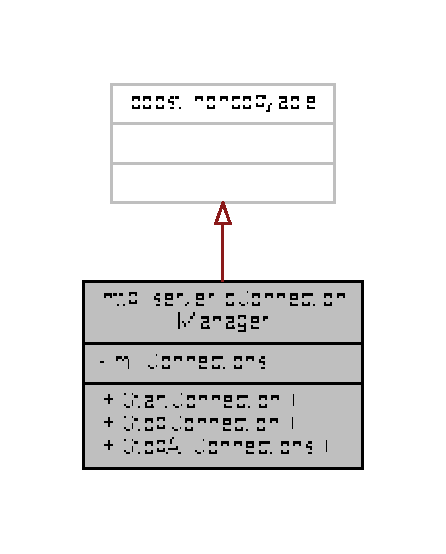
\includegraphics[width=214pt]{classhttp__server_1_1cConnectionManager__inherit__graph}
\end{center}
\end{figure}


Collaboration diagram for http\-\_\-server\-:\-:c\-Connection\-Manager\-:
\nopagebreak
\begin{figure}[H]
\begin{center}
\leavevmode
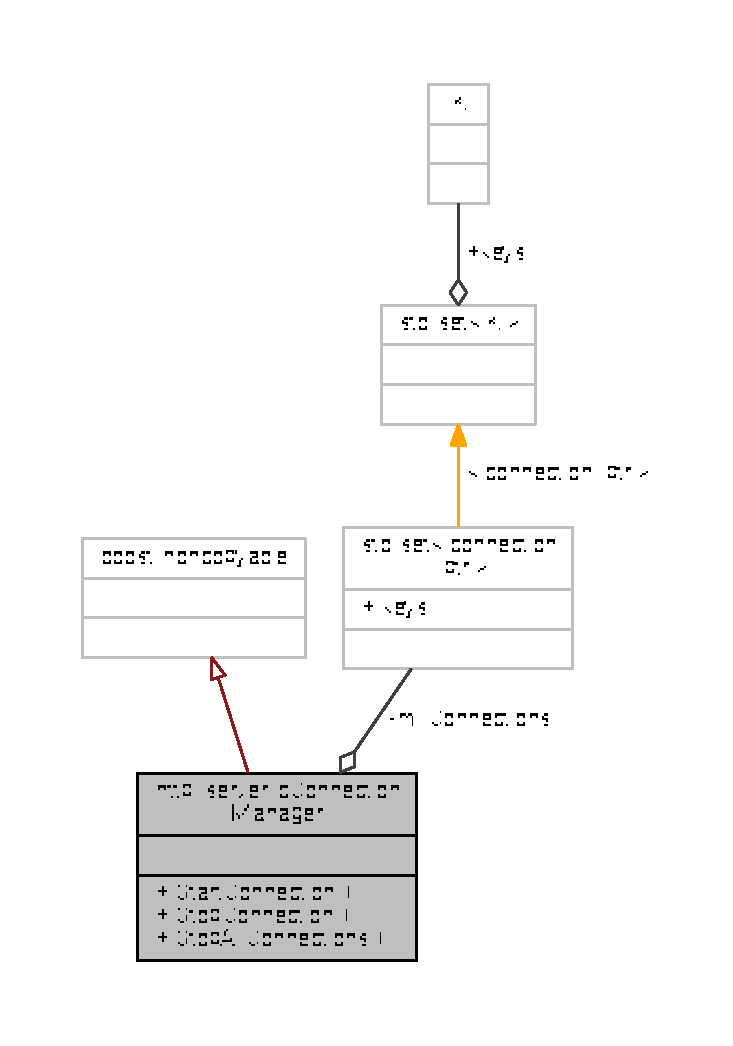
\includegraphics[width=350pt]{classhttp__server_1_1cConnectionManager__coll__graph}
\end{center}
\end{figure}
\subsection*{Public Member Functions}
\begin{DoxyCompactItemize}
\item 
\hypertarget{classhttp__server_1_1cConnectionManager_ab7741005e29b740894addaded7a17ee2}{void {\bfseries Start\-Connection} (connection\-\_\-ptr)}\label{classhttp__server_1_1cConnectionManager_ab7741005e29b740894addaded7a17ee2}

\item 
\hypertarget{classhttp__server_1_1cConnectionManager_a740f1202cf4db1493aac3c8f0a99bbb4}{void {\bfseries Stop\-Connection} (connection\-\_\-ptr)}\label{classhttp__server_1_1cConnectionManager_a740f1202cf4db1493aac3c8f0a99bbb4}

\item 
\hypertarget{classhttp__server_1_1cConnectionManager_a5dddb041d33c7bbb4220deaa9dd74b3c}{void {\bfseries Stop\-All\-Connections} ()}\label{classhttp__server_1_1cConnectionManager_a5dddb041d33c7bbb4220deaa9dd74b3c}

\end{DoxyCompactItemize}
\subsection*{Private Attributes}
\begin{DoxyCompactItemize}
\item 
\hypertarget{classhttp__server_1_1cConnectionManager_a6bc3632311d979511b8393d611b88752}{std\-::set$<$ connection\-\_\-ptr $>$ {\bfseries m\-\_\-\-Connections}}\label{classhttp__server_1_1cConnectionManager_a6bc3632311d979511b8393d611b88752}

\end{DoxyCompactItemize}


\subsection{Detailed Description}
class that maintains a a set of connections 

The documentation for this class was generated from the following files\-:\begin{DoxyCompactItemize}
\item 
connection\-\_\-manager.\-h\item 
connection\-\_\-manager.\-cpp\end{DoxyCompactItemize}

\hypertarget{classhttp__server_1_1cHeader}{\section{http\-\_\-server\-:\-:c\-Header Class Reference}
\label{classhttp__server_1_1cHeader}\index{http\-\_\-server\-::c\-Header@{http\-\_\-server\-::c\-Header}}
}


Collaboration diagram for http\-\_\-server\-:\-:c\-Header\-:
\subsection*{Public Member Functions}
\begin{DoxyCompactItemize}
\item 
\hypertarget{classhttp__server_1_1cHeader_a0da2d042d4c8377ab03e5e5db07e9851}{{\bfseries c\-Header} (std\-::string \&header)}\label{classhttp__server_1_1cHeader_a0da2d042d4c8377ab03e5e5db07e9851}

\end{DoxyCompactItemize}
\subsection*{Private Attributes}
\begin{DoxyCompactItemize}
\item 
\hypertarget{classhttp__server_1_1cHeader_ae240317901e48fb784522ecfdd0187f1}{std\-::string {\bfseries m\-\_\-\-Header}}\label{classhttp__server_1_1cHeader_ae240317901e48fb784522ecfdd0187f1}

\item 
\hypertarget{classhttp__server_1_1cHeader_a549796c5afa30e103a14e69ce68bedab}{H\-E\-A\-D\-E\-R\-\_\-\-T\-Y\-P\-E {\bfseries m\-\_\-\-Header\-Type}}\label{classhttp__server_1_1cHeader_a549796c5afa30e103a14e69ce68bedab}

\end{DoxyCompactItemize}


The documentation for this class was generated from the following file\-:\begin{DoxyCompactItemize}
\item 
http\-\_\-header.\-h\end{DoxyCompactItemize}

\hypertarget{classhttp__server_1_1cHttpConnection}{\section{http\-\_\-server\-:\-:c\-Http\-Connection \-Class \-Reference}
\label{classhttp__server_1_1cHttpConnection}\index{http\-\_\-server\-::c\-Http\-Connection@{http\-\_\-server\-::c\-Http\-Connection}}
}


\-Collaboration diagram for http\-\_\-server\-:\-:c\-Http\-Connection\-:\nopagebreak
\begin{figure}[H]
\begin{center}
\leavevmode
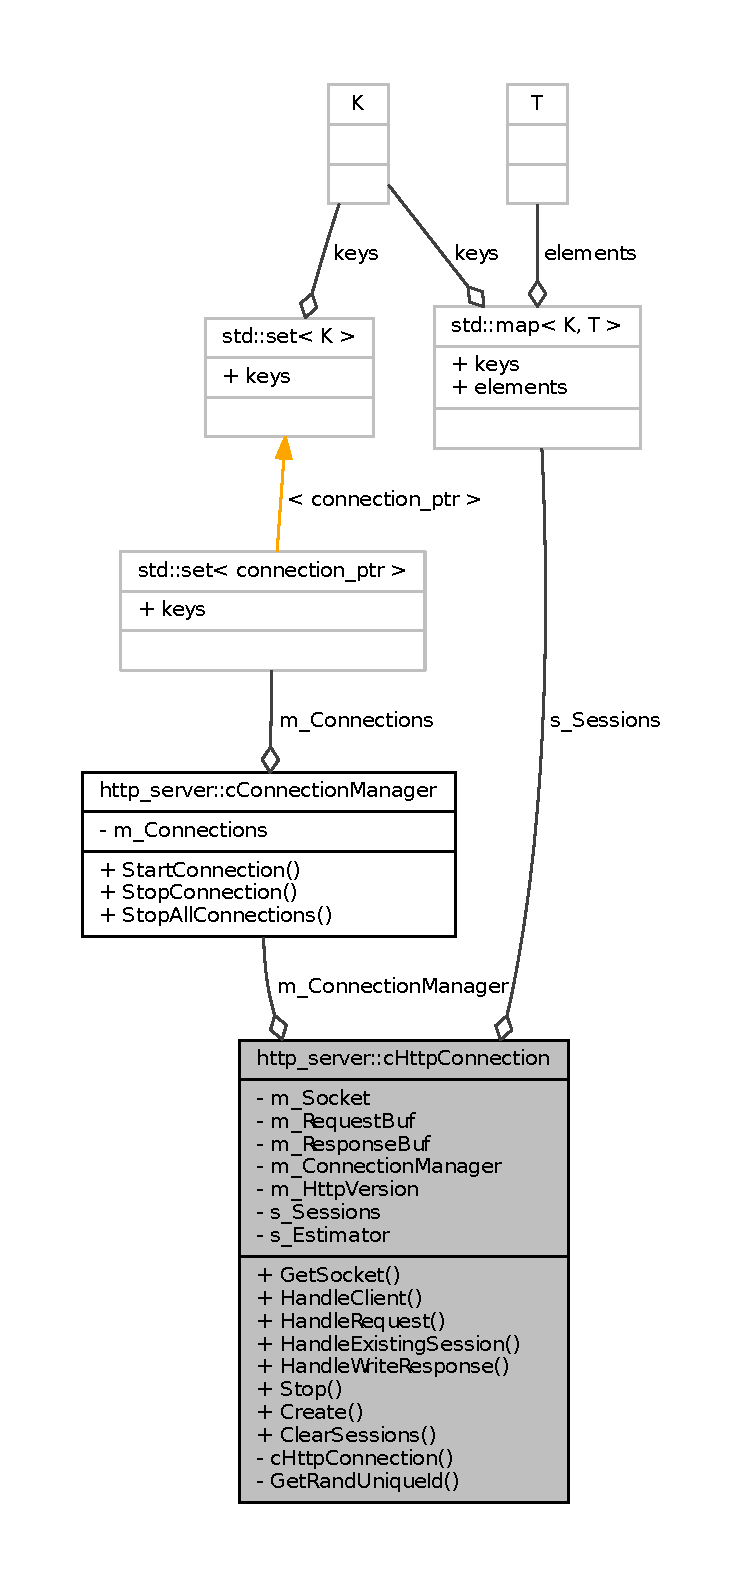
\includegraphics[height=550pt]{classhttp__server_1_1cHttpConnection__coll__graph}
\end{center}
\end{figure}
\subsection*{\-Public \-Member \-Functions}
\begin{DoxyCompactItemize}
\item 
\hypertarget{classhttp__server_1_1cHttpConnection_ad9175494a963a2e2f7fafb31c24c4783}{boost\-::asio\-::ip\-::tcp\-::socket \& {\bfseries \-Get\-Socket} ()}\label{classhttp__server_1_1cHttpConnection_ad9175494a963a2e2f7fafb31c24c4783}

\item 
\hypertarget{classhttp__server_1_1cHttpConnection_a0559eb591a884a16d90f2e061a5530f6}{void {\bfseries \-Handle\-Client} ()}\label{classhttp__server_1_1cHttpConnection_a0559eb591a884a16d90f2e061a5530f6}

\item 
\hypertarget{classhttp__server_1_1cHttpConnection_aad4d12163015ab391b40bb15b9a5ecb0}{void {\bfseries \-Handle\-Request} (const boost\-::system\-::error\-\_\-code \&error)}\label{classhttp__server_1_1cHttpConnection_aad4d12163015ab391b40bb15b9a5ecb0}

\item 
\hypertarget{classhttp__server_1_1cHttpConnection_aa9343fd8557891c23c8fd73b5641fedd}{void {\bfseries \-Handle\-Existing\-Session} (\hyperlink{classhttp__server_1_1cResponse}{c\-Response} \&response, const \hyperlink{classhttp__server_1_1cRequest}{c\-Request} \&\-\_\-request, const unsigned int ses\-\_\-id)}\label{classhttp__server_1_1cHttpConnection_aa9343fd8557891c23c8fd73b5641fedd}

\item 
\hypertarget{classhttp__server_1_1cHttpConnection_a128cc40027898c87335516147b767b87}{void {\bfseries \-Handle\-Write\-Response} (const boost\-::system\-::error\-\_\-code \&error)}\label{classhttp__server_1_1cHttpConnection_a128cc40027898c87335516147b767b87}

\item 
\hypertarget{classhttp__server_1_1cHttpConnection_aac06a1408cb3b2e20e08817858e45443}{void {\bfseries \-Stop} ()}\label{classhttp__server_1_1cHttpConnection_aac06a1408cb3b2e20e08817858e45443}

\end{DoxyCompactItemize}
\subsection*{\-Static \-Public \-Member \-Functions}
\begin{DoxyCompactItemize}
\item 
\hypertarget{classhttp__server_1_1cHttpConnection_a03b465f45c06bcc42c3a4e771ab00395}{static connection\-\_\-ptr {\bfseries \-Create} (boost\-::asio\-::io\-\_\-service \&io\-\_\-service, \hyperlink{classhttp__server_1_1cConnectionManager}{c\-Connection\-Manager} \&conn\-\_\-manager)}\label{classhttp__server_1_1cHttpConnection_a03b465f45c06bcc42c3a4e771ab00395}

\item 
\hypertarget{classhttp__server_1_1cHttpConnection_a233c74cfb8a64cfb93be34e2fca92741}{static void {\bfseries \-Clear\-Sessions} ()}\label{classhttp__server_1_1cHttpConnection_a233c74cfb8a64cfb93be34e2fca92741}

\end{DoxyCompactItemize}
\subsection*{\-Private \-Types}
\begin{DoxyCompactItemize}
\item 
\hypertarget{classhttp__server_1_1cHttpConnection_a0a5b09ba857189a7f7179096fdb15c09}{typedef boost\-::shared\-\_\-ptr\*
$<$ \hyperlink{classhttp__server_1_1cHttpConnection}{c\-Http\-Connection} $>$ {\bfseries connection\-\_\-ptr}}\label{classhttp__server_1_1cHttpConnection_a0a5b09ba857189a7f7179096fdb15c09}

\item 
\hypertarget{classhttp__server_1_1cHttpConnection_aef12353a1c35536062088868a1c47d16}{typedef std\-::map$<$ unsigned int, \*
engine\-::c\-Session $\ast$ $>$ {\bfseries sessions\-\_\-map}}\label{classhttp__server_1_1cHttpConnection_aef12353a1c35536062088868a1c47d16}

\end{DoxyCompactItemize}
\subsection*{\-Private \-Member \-Functions}
\begin{DoxyCompactItemize}
\item 
\hypertarget{classhttp__server_1_1cHttpConnection_a8b0305459f933592f64fab2e3289dd54}{{\bfseries c\-Http\-Connection} (boost\-::asio\-::io\-\_\-service \&io\-\_\-service, \hyperlink{classhttp__server_1_1cConnectionManager}{c\-Connection\-Manager} \&conn\-\_\-manager)}\label{classhttp__server_1_1cHttpConnection_a8b0305459f933592f64fab2e3289dd54}

\end{DoxyCompactItemize}
\subsection*{\-Static \-Private \-Member \-Functions}
\begin{DoxyCompactItemize}
\item 
\hypertarget{classhttp__server_1_1cHttpConnection_ae4193c0d2fcd91ee80849f0982b4fe14}{static unsigned int {\bfseries \-Get\-Rand\-Unique\-Id} ()}\label{classhttp__server_1_1cHttpConnection_ae4193c0d2fcd91ee80849f0982b4fe14}

\end{DoxyCompactItemize}
\subsection*{\-Private \-Attributes}
\begin{DoxyCompactItemize}
\item 
\hypertarget{classhttp__server_1_1cHttpConnection_acf6b64550b0e0f8287d7b55a5613ef0f}{boost\-::asio\-::ip\-::tcp\-::socket {\bfseries m\-\_\-\-Socket}}\label{classhttp__server_1_1cHttpConnection_acf6b64550b0e0f8287d7b55a5613ef0f}

\item 
\hypertarget{classhttp__server_1_1cHttpConnection_a0504245e3903f238ff13145a832d4582}{boost\-::asio\-::streambuf {\bfseries m\-\_\-\-Request\-Buf}}\label{classhttp__server_1_1cHttpConnection_a0504245e3903f238ff13145a832d4582}

\item 
\hypertarget{classhttp__server_1_1cHttpConnection_a6f99bd0fa66b31461010ef0948fa428f}{boost\-::asio\-::streambuf {\bfseries m\-\_\-\-Response\-Buf}}\label{classhttp__server_1_1cHttpConnection_a6f99bd0fa66b31461010ef0948fa428f}

\item 
\hypertarget{classhttp__server_1_1cHttpConnection_adea2cf9ab3ff28fd70c9a910ef9bfda3}{\hyperlink{classhttp__server_1_1cConnectionManager}{c\-Connection\-Manager} \& {\bfseries m\-\_\-\-Connection\-Manager}}\label{classhttp__server_1_1cHttpConnection_adea2cf9ab3ff28fd70c9a910ef9bfda3}

\item 
\hypertarget{classhttp__server_1_1cHttpConnection_a785dff3fa5be6e114762738aae4d031e}{bool {\bfseries m\-\_\-\-Http\-Version}}\label{classhttp__server_1_1cHttpConnection_a785dff3fa5be6e114762738aae4d031e}

\end{DoxyCompactItemize}
\subsection*{\-Static \-Private \-Attributes}
\begin{DoxyCompactItemize}
\item 
\hypertarget{classhttp__server_1_1cHttpConnection_a1d3d86ae704fe225d6420d6d6fd7340e}{static sessions\-\_\-map {\bfseries s\-\_\-\-Sessions}}\label{classhttp__server_1_1cHttpConnection_a1d3d86ae704fe225d6420d6d6fd7340e}

\item 
\hypertarget{classhttp__server_1_1cHttpConnection_ae1b6b9bb43bb406ce4c9e9f027348263}{static engine\-::c\-Estimator {\bfseries s\-\_\-\-Estimator}}\label{classhttp__server_1_1cHttpConnection_ae1b6b9bb43bb406ce4c9e9f027348263}

\end{DoxyCompactItemize}


\-The documentation for this class was generated from the following files\-:\begin{DoxyCompactItemize}
\item 
http\-\_\-connection.\-h\item 
http\-\_\-connection.\-cpp\end{DoxyCompactItemize}

\hypertarget{classhttp__server_1_1cHttpServer}{\section{http\-\_\-server\-:\-:c\-Http\-Server \-Class \-Reference}
\label{classhttp__server_1_1cHttpServer}\index{http\-\_\-server\-::c\-Http\-Server@{http\-\_\-server\-::c\-Http\-Server}}
}


{\ttfamily \#include $<$http\-\_\-server.\-h$>$}



\-Collaboration diagram for http\-\_\-server\-:\-:c\-Http\-Server\-:
\nopagebreak
\begin{figure}[H]
\begin{center}
\leavevmode
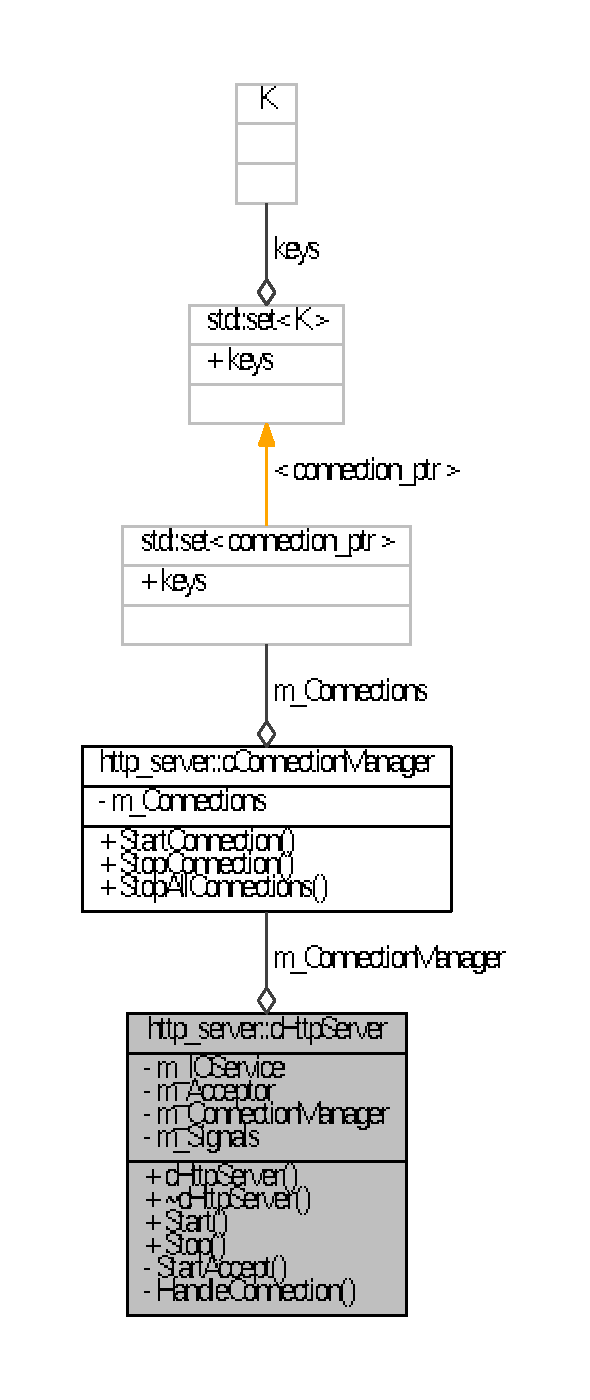
\includegraphics[height=550pt]{classhttp__server_1_1cHttpServer__coll__graph}
\end{center}
\end{figure}
\subsection*{\-Public \-Member \-Functions}
\begin{DoxyCompactItemize}
\item 
\hyperlink{classhttp__server_1_1cHttpServer_a26d917897dda50502ea1469fb5af9c2e}{c\-Http\-Server} (unsigned int port)
\item 
\hyperlink{classhttp__server_1_1cHttpServer_a783dd5b31b19b8a95e6c2ce7c188a7c9}{$\sim$c\-Http\-Server} ()
\item 
void \hyperlink{classhttp__server_1_1cHttpServer_ad4699b20627615aee961a06eae97fb89}{\-Start} ()
\item 
void \hyperlink{classhttp__server_1_1cHttpServer_a2c7bcb8fb8ca1aa5fe26d00c94c11835}{\-Stop} ()
\end{DoxyCompactItemize}
\subsection*{\-Private \-Member \-Functions}
\begin{DoxyCompactItemize}
\item 
\hypertarget{classhttp__server_1_1cHttpServer_abec1513422a3b70b8c3684f4dc8c6271}{void {\bfseries \-Start\-Accept} ()}\label{classhttp__server_1_1cHttpServer_abec1513422a3b70b8c3684f4dc8c6271}

\item 
\hypertarget{classhttp__server_1_1cHttpServer_adfe4c5b575c0e94174a64d228f152d46}{void {\bfseries \-Handle\-Connection} (connection\-\_\-ptr new\-\_\-connection, const boost\-::system\-::error\-\_\-code \&error)}\label{classhttp__server_1_1cHttpServer_adfe4c5b575c0e94174a64d228f152d46}

\end{DoxyCompactItemize}
\subsection*{\-Private \-Attributes}
\begin{DoxyCompactItemize}
\item 
\hypertarget{classhttp__server_1_1cHttpServer_ae02a73720c1b0fa45b787ef0cecacb6c}{boost\-::asio\-::io\-\_\-service {\bfseries m\-\_\-\-I\-O\-Service}}\label{classhttp__server_1_1cHttpServer_ae02a73720c1b0fa45b787ef0cecacb6c}

\item 
\hypertarget{classhttp__server_1_1cHttpServer_a2d4db5bec75f0594e81403e8659ec2a0}{boost\-::asio\-::ip\-::tcp\-::acceptor {\bfseries m\-\_\-\-Acceptor}}\label{classhttp__server_1_1cHttpServer_a2d4db5bec75f0594e81403e8659ec2a0}

\item 
\hypertarget{classhttp__server_1_1cHttpServer_a87a2959bcad40f733bb9bd79f03bc017}{\hyperlink{classhttp__server_1_1cConnectionManager}{c\-Connection\-Manager} {\bfseries m\-\_\-\-Connection\-Manager}}\label{classhttp__server_1_1cHttpServer_a87a2959bcad40f733bb9bd79f03bc017}

\item 
\hypertarget{classhttp__server_1_1cHttpServer_a6332aa8cd965ba14ee125d90e309c483}{boost\-::asio\-::signal\-\_\-set {\bfseries m\-\_\-\-Signals}}\label{classhttp__server_1_1cHttpServer_a6332aa8cd965ba14ee125d90e309c483}

\end{DoxyCompactItemize}


\subsection{\-Detailed \-Description}
class that implements a http server using \-B\-O\-O\-S\-T \-A\-S\-I\-O 

\subsection{\-Constructor \& \-Destructor \-Documentation}
\hypertarget{classhttp__server_1_1cHttpServer_a26d917897dda50502ea1469fb5af9c2e}{\index{http\-\_\-server\-::c\-Http\-Server@{http\-\_\-server\-::c\-Http\-Server}!c\-Http\-Server@{c\-Http\-Server}}
\index{c\-Http\-Server@{c\-Http\-Server}!http_server::cHttpServer@{http\-\_\-server\-::c\-Http\-Server}}
\subsubsection[{c\-Http\-Server}]{\setlength{\rightskip}{0pt plus 5cm}{\bf http\-\_\-server\-::c\-Http\-Server\-::c\-Http\-Server} (
\begin{DoxyParamCaption}
\item[{unsigned int}]{port}
\end{DoxyParamCaption}
)}}\label{classhttp__server_1_1cHttpServer_a26d917897dda50502ea1469fb5af9c2e}
initializes members and prepares for accepting connections 

\-Here is the call graph for this function\-:
\nopagebreak
\begin{figure}[H]
\begin{center}
\leavevmode
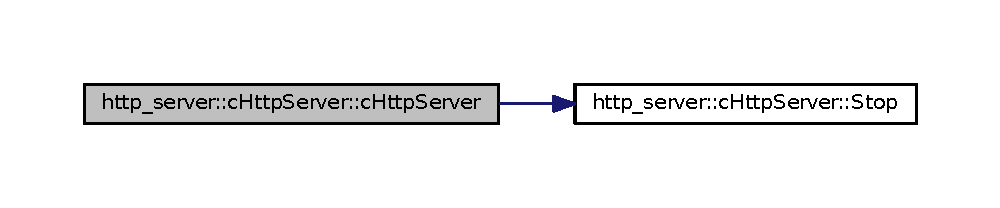
\includegraphics[width=350pt]{classhttp__server_1_1cHttpServer_a26d917897dda50502ea1469fb5af9c2e_cgraph}
\end{center}
\end{figure}


\hypertarget{classhttp__server_1_1cHttpServer_a783dd5b31b19b8a95e6c2ce7c188a7c9}{\index{http\-\_\-server\-::c\-Http\-Server@{http\-\_\-server\-::c\-Http\-Server}!$\sim$c\-Http\-Server@{$\sim$c\-Http\-Server}}
\index{$\sim$c\-Http\-Server@{$\sim$c\-Http\-Server}!http_server::cHttpServer@{http\-\_\-server\-::c\-Http\-Server}}
\subsubsection[{$\sim$c\-Http\-Server}]{\setlength{\rightskip}{0pt plus 5cm}{\bf http\-\_\-server\-::c\-Http\-Server\-::$\sim$c\-Http\-Server} (
\begin{DoxyParamCaption}
{}
\end{DoxyParamCaption}
)}}\label{classhttp__server_1_1cHttpServer_a783dd5b31b19b8a95e6c2ce7c188a7c9}
stops the server 

\-Here is the call graph for this function\-:
\nopagebreak
\begin{figure}[H]
\begin{center}
\leavevmode
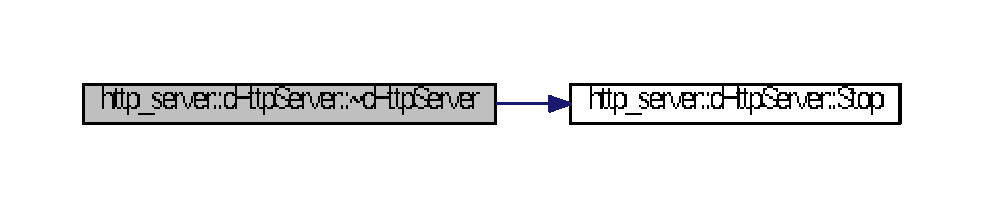
\includegraphics[width=350pt]{classhttp__server_1_1cHttpServer_a783dd5b31b19b8a95e6c2ce7c188a7c9_cgraph}
\end{center}
\end{figure}




\subsection{\-Member \-Function \-Documentation}
\hypertarget{classhttp__server_1_1cHttpServer_ad4699b20627615aee961a06eae97fb89}{\index{http\-\_\-server\-::c\-Http\-Server@{http\-\_\-server\-::c\-Http\-Server}!\-Start@{\-Start}}
\index{\-Start@{\-Start}!http_server::cHttpServer@{http\-\_\-server\-::c\-Http\-Server}}
\subsubsection[{\-Start}]{\setlength{\rightskip}{0pt plus 5cm}void {\bf http\-\_\-server\-::c\-Http\-Server\-::\-Start} (
\begin{DoxyParamCaption}
{}
\end{DoxyParamCaption}
)}}\label{classhttp__server_1_1cHttpServer_ad4699b20627615aee961a06eae97fb89}
starts the server \hypertarget{classhttp__server_1_1cHttpServer_a2c7bcb8fb8ca1aa5fe26d00c94c11835}{\index{http\-\_\-server\-::c\-Http\-Server@{http\-\_\-server\-::c\-Http\-Server}!\-Stop@{\-Stop}}
\index{\-Stop@{\-Stop}!http_server::cHttpServer@{http\-\_\-server\-::c\-Http\-Server}}
\subsubsection[{\-Stop}]{\setlength{\rightskip}{0pt plus 5cm}void {\bf http\-\_\-server\-::c\-Http\-Server\-::\-Stop} (
\begin{DoxyParamCaption}
{}
\end{DoxyParamCaption}
)}}\label{classhttp__server_1_1cHttpServer_a2c7bcb8fb8ca1aa5fe26d00c94c11835}
stops the server 

\-The documentation for this class was generated from the following files\-:\begin{DoxyCompactItemize}
\item 
http\-\_\-server.\-h\item 
http\-\_\-server.\-cpp\end{DoxyCompactItemize}

\hypertarget{structhttp__server_1_1command__}{\section{http\-\_\-server\-:\-:command\-\_\- \-Struct \-Reference}
\label{structhttp__server_1_1command__}\index{http\-\_\-server\-::command\-\_\-@{http\-\_\-server\-::command\-\_\-}}
}


\-The documentation for this struct was generated from the following file\-:\begin{DoxyCompactItemize}
\item 
http\-\_\-request.\-cpp\end{DoxyCompactItemize}

\hypertarget{classhttp__server_1_1cPageBuilder}{\section{http\-\_\-server\-:\-:c\-Page\-Builder \-Class \-Reference}
\label{classhttp__server_1_1cPageBuilder}\index{http\-\_\-server\-::c\-Page\-Builder@{http\-\_\-server\-::c\-Page\-Builder}}
}


\-Collaboration diagram for http\-\_\-server\-:\-:c\-Page\-Builder\-:\nopagebreak
\begin{figure}[H]
\begin{center}
\leavevmode
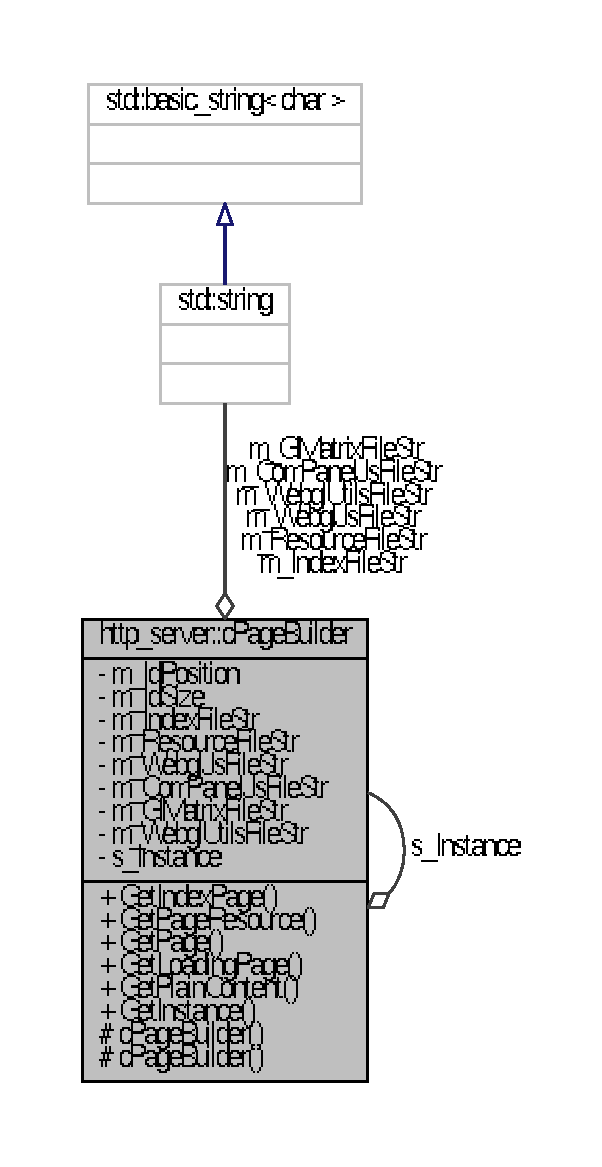
\includegraphics[height=550pt]{classhttp__server_1_1cPageBuilder__coll__graph}
\end{center}
\end{figure}
\subsection*{\-Public \-Member \-Functions}
\begin{DoxyCompactItemize}
\item 
\hypertarget{classhttp__server_1_1cPageBuilder_aad87a17faa8505727c8faac59a7a9674}{const std\-::string \& {\bfseries \-Get\-Index\-Page} (const unsigned int session\-\_\-id)}\label{classhttp__server_1_1cPageBuilder_aad87a17faa8505727c8faac59a7a9674}

\item 
\hypertarget{classhttp__server_1_1cPageBuilder_ac7a52ef639767e3f9297376cced2a8ab}{const std\-::string \& {\bfseries \-Get\-Page\-Resource} (const std\-::string \&resource) const }\label{classhttp__server_1_1cPageBuilder_ac7a52ef639767e3f9297376cced2a8ab}

\item 
\hypertarget{classhttp__server_1_1cPageBuilder_a399e3fcab5b631e64907a183af1e8b44}{const std\-::string {\bfseries \-Get\-Page} (const engine\-::c\-Result \&result, const unsigned int ses\-\_\-id) const }\label{classhttp__server_1_1cPageBuilder_a399e3fcab5b631e64907a183af1e8b44}

\item 
\hypertarget{classhttp__server_1_1cPageBuilder_a903fe3604f402c70bd04aefbbe322cbc}{const std\-::string {\bfseries \-Get\-Loading\-Page} (const unsigned int estimation, const unsigned int ses\-\_\-id) const }\label{classhttp__server_1_1cPageBuilder_a903fe3604f402c70bd04aefbbe322cbc}

\item 
\hypertarget{classhttp__server_1_1cPageBuilder_a1d94480e16491f15aa3ed974dfb181e1}{const std\-::string {\bfseries \-Get\-Plain\-Content} (const std\-::string \&planecontent) const }\label{classhttp__server_1_1cPageBuilder_a1d94480e16491f15aa3ed974dfb181e1}

\end{DoxyCompactItemize}
\subsection*{\-Static \-Public \-Member \-Functions}
\begin{DoxyCompactItemize}
\item 
\hypertarget{classhttp__server_1_1cPageBuilder_acf7940105f1b4f5d77a0cecac9a69db6}{static \hyperlink{classhttp__server_1_1cPageBuilder}{c\-Page\-Builder} $\ast$ {\bfseries \-Get\-Instance} ()}\label{classhttp__server_1_1cPageBuilder_acf7940105f1b4f5d77a0cecac9a69db6}

\end{DoxyCompactItemize}
\subsection*{\-Protected \-Member \-Functions}
\begin{DoxyCompactItemize}
\item 
\hypertarget{classhttp__server_1_1cPageBuilder_a3f3d04425b2f912c5616362b9be5d19e}{{\bfseries c\-Page\-Builder} (const \hyperlink{classhttp__server_1_1cPageBuilder}{c\-Page\-Builder} \&page\-\_\-bld)}\label{classhttp__server_1_1cPageBuilder_a3f3d04425b2f912c5616362b9be5d19e}

\end{DoxyCompactItemize}
\subsection*{\-Private \-Attributes}
\begin{DoxyCompactItemize}
\item 
\hypertarget{classhttp__server_1_1cPageBuilder_a98fc3701625a6e09deb368eca4aae6da}{std\-::size\-\_\-t {\bfseries m\-\_\-\-Id\-Position}}\label{classhttp__server_1_1cPageBuilder_a98fc3701625a6e09deb368eca4aae6da}

\item 
\hypertarget{classhttp__server_1_1cPageBuilder_a2a5da5d3ab0f9f61046e2111ea36b039}{std\-::size\-\_\-t {\bfseries m\-\_\-\-Id\-Size}}\label{classhttp__server_1_1cPageBuilder_a2a5da5d3ab0f9f61046e2111ea36b039}

\item 
\hypertarget{classhttp__server_1_1cPageBuilder_a2c4b56ac0d42ba3d9d20945839082ef5}{std\-::string {\bfseries m\-\_\-\-Index\-File\-Str}}\label{classhttp__server_1_1cPageBuilder_a2c4b56ac0d42ba3d9d20945839082ef5}

\item 
\hypertarget{classhttp__server_1_1cPageBuilder_adc3bb5aec5159c7556a6012562faf9f0}{std\-::string {\bfseries m\-\_\-\-Resource\-File\-Str}}\label{classhttp__server_1_1cPageBuilder_adc3bb5aec5159c7556a6012562faf9f0}

\item 
\hypertarget{classhttp__server_1_1cPageBuilder_ab042991bd624949e0a45d62e975dacdd}{std\-::string {\bfseries m\-\_\-\-Webgl\-Js\-File\-Str}}\label{classhttp__server_1_1cPageBuilder_ab042991bd624949e0a45d62e975dacdd}

\item 
\hypertarget{classhttp__server_1_1cPageBuilder_acff93f71f4bbc839dba06b1732ea3fa2}{std\-::string {\bfseries m\-\_\-\-Com\-Panel\-Js\-File\-Str}}\label{classhttp__server_1_1cPageBuilder_acff93f71f4bbc839dba06b1732ea3fa2}

\item 
\hypertarget{classhttp__server_1_1cPageBuilder_abc5defb9eaf551d6e2b8334bb0576693}{std\-::string {\bfseries m\-\_\-\-Gl\-Matrix\-File\-Str}}\label{classhttp__server_1_1cPageBuilder_abc5defb9eaf551d6e2b8334bb0576693}

\item 
\hypertarget{classhttp__server_1_1cPageBuilder_a20f28a3a4f2a8e42f06544bdb8e22058}{std\-::string {\bfseries m\-\_\-\-Webgl\-Utils\-File\-Str}}\label{classhttp__server_1_1cPageBuilder_a20f28a3a4f2a8e42f06544bdb8e22058}

\end{DoxyCompactItemize}
\subsection*{\-Static \-Private \-Attributes}
\begin{DoxyCompactItemize}
\item 
\hypertarget{classhttp__server_1_1cPageBuilder_a5857987a8133c3768bac833850d12613}{static \hyperlink{classhttp__server_1_1cPageBuilder}{c\-Page\-Builder} $\ast$ {\bfseries s\-\_\-\-Instance} = \-N\-U\-L\-L}\label{classhttp__server_1_1cPageBuilder_a5857987a8133c3768bac833850d12613}

\end{DoxyCompactItemize}


\-The documentation for this class was generated from the following files\-:\begin{DoxyCompactItemize}
\item 
pagebuilder.\-h\item 
pagebuilder.\-cpp\end{DoxyCompactItemize}

\hypertarget{classhttp__server_1_1cRequest}{\section{http\-\_\-server\-:\-:c\-Request Class Reference}
\label{classhttp__server_1_1cRequest}\index{http\-\_\-server\-::c\-Request@{http\-\_\-server\-::c\-Request}}
}


Collaboration diagram for http\-\_\-server\-:\-:c\-Request\-:
\subsection*{Public Member Functions}
\begin{DoxyCompactItemize}
\item 
\hypertarget{classhttp__server_1_1cRequest_aa3cadbdda5c1ad42a29f182bddc94fb1}{{\bfseries c\-Request} (std\-::istream \&stream)}\label{classhttp__server_1_1cRequest_aa3cadbdda5c1ad42a29f182bddc94fb1}

\item 
\hypertarget{classhttp__server_1_1cRequest_ac9531a813f05222ee24c7a27d2ec90fd}{bool {\bfseries Parse\-Request} ()}\label{classhttp__server_1_1cRequest_ac9531a813f05222ee24c7a27d2ec90fd}

\item 
\hypertarget{classhttp__server_1_1cRequest_ab623c396e4dbde0253c99c0a609f275f}{bool {\bfseries Parse\-Resource} ()}\label{classhttp__server_1_1cRequest_ab623c396e4dbde0253c99c0a609f275f}

\item 
\hypertarget{classhttp__server_1_1cRequest_a4526de1f0c6af63f325b540fa763330b}{std\-::vector$<$ \hyperlink{classhttp__server_1_1cHeader}{c\-Header} $\ast$ $>$ {\bfseries Parse\-Headers} ()}\label{classhttp__server_1_1cRequest_a4526de1f0c6af63f325b540fa763330b}

\item 
\hypertarget{classhttp__server_1_1cRequest_af0c3d838c88fef758115eda75cd66835}{R\-E\-Q\-\_\-\-M\-E\-T\-H\-O\-D {\bfseries Get\-Method} () const }\label{classhttp__server_1_1cRequest_af0c3d838c88fef758115eda75cd66835}

\item 
\hypertarget{classhttp__server_1_1cRequest_a808d2f736c751db6d111d2cbb2458470}{const std\-::string \& {\bfseries Get\-Resource} () const }\label{classhttp__server_1_1cRequest_a808d2f736c751db6d111d2cbb2458470}

\item 
\hypertarget{classhttp__server_1_1cRequest_a9f1fbe83f22a917f75085326b96a5577}{const std\-::string \& {\bfseries Get\-Version} () const }\label{classhttp__server_1_1cRequest_a9f1fbe83f22a917f75085326b96a5577}

\item 
\hypertarget{classhttp__server_1_1cRequest_a51ccd6f85abf1eb131bd3e2c10ad2f59}{C\-O\-M\-M\-A\-N\-D\-\_\-\-T\-Y\-P\-E {\bfseries Get\-Command\-Id} () const }\label{classhttp__server_1_1cRequest_a51ccd6f85abf1eb131bd3e2c10ad2f59}

\item 
\hypertarget{classhttp__server_1_1cRequest_a386946841d675edc9dbf5fd81d8de046}{const std\-::string \& {\bfseries Get\-Param} () const }\label{classhttp__server_1_1cRequest_a386946841d675edc9dbf5fd81d8de046}

\item 
\hypertarget{classhttp__server_1_1cRequest_ada8f38975ca9bb05bfe9b5b34aa985a5}{const unsigned int {\bfseries Get\-Session\-Id} () const }\label{classhttp__server_1_1cRequest_ada8f38975ca9bb05bfe9b5b34aa985a5}

\end{DoxyCompactItemize}
\subsection*{Private Types}
\begin{DoxyCompactItemize}
\item 
\hypertarget{classhttp__server_1_1cRequest_ab55878881ea0fad5b7801a7d3e67bc6f}{typedef \\*
std\-::istreambuf\-\_\-iterator$<$ char $>$ {\bfseries base\-\_\-iterator\-\_\-type}}\label{classhttp__server_1_1cRequest_ab55878881ea0fad5b7801a7d3e67bc6f}

\item 
\hypertarget{classhttp__server_1_1cRequest_a4c4ef5da2042acec5d8f9ff9f0a432c3}{typedef \\*
boost\-::spirit\-::multi\-\_\-pass\\*
$<$ base\-\_\-iterator\-\_\-type $>$ {\bfseries forward\-\_\-iterator\-\_\-type}}\label{classhttp__server_1_1cRequest_a4c4ef5da2042acec5d8f9ff9f0a432c3}

\end{DoxyCompactItemize}
\subsection*{Private Attributes}
\begin{DoxyCompactItemize}
\item 
\hypertarget{classhttp__server_1_1cRequest_a4702912c2025f7ce153f9ac68567b55c}{R\-E\-Q\-\_\-\-M\-E\-T\-H\-O\-D {\bfseries m\-\_\-\-Method}}\label{classhttp__server_1_1cRequest_a4702912c2025f7ce153f9ac68567b55c}

\item 
\hypertarget{classhttp__server_1_1cRequest_a4bd223196a1aa78de6ff2de4202232fa}{std\-::string {\bfseries m\-\_\-\-Resource}}\label{classhttp__server_1_1cRequest_a4bd223196a1aa78de6ff2de4202232fa}

\item 
\hypertarget{classhttp__server_1_1cRequest_ab64ead387c97768aabc1bed343731153}{std\-::string {\bfseries m\-\_\-\-Version}}\label{classhttp__server_1_1cRequest_ab64ead387c97768aabc1bed343731153}

\item 
\hypertarget{classhttp__server_1_1cRequest_aa1e6a65858e9cf26432add99470e4104}{std\-::string {\bfseries m\-\_\-\-Headers}}\label{classhttp__server_1_1cRequest_aa1e6a65858e9cf26432add99470e4104}

\item 
\hypertarget{classhttp__server_1_1cRequest_a2481a39733ba13124de865b30598a310}{C\-O\-M\-M\-A\-N\-D\-\_\-\-T\-Y\-P\-E {\bfseries m\-\_\-\-Command\-Id}}\label{classhttp__server_1_1cRequest_a2481a39733ba13124de865b30598a310}

\item 
\hypertarget{classhttp__server_1_1cRequest_a5320d5862827483c3f72c4fb385bcb16}{std\-::string {\bfseries m\-\_\-\-Param}}\label{classhttp__server_1_1cRequest_a5320d5862827483c3f72c4fb385bcb16}

\item 
\hypertarget{classhttp__server_1_1cRequest_a9c32df40a547799225a5ec41099fde53}{unsigned int {\bfseries m\-\_\-\-Session\-Id}}\label{classhttp__server_1_1cRequest_a9c32df40a547799225a5ec41099fde53}

\item 
\hypertarget{classhttp__server_1_1cRequest_a346ff4a99509f28178aa3702a877d438}{forward\-\_\-iterator\-\_\-type {\bfseries m\-\_\-\-Fwd\-\_\-begin}}\label{classhttp__server_1_1cRequest_a346ff4a99509f28178aa3702a877d438}

\item 
\hypertarget{classhttp__server_1_1cRequest_ad9fb0f78ed6fca01cdcdc6b3b01ba519}{forward\-\_\-iterator\-\_\-type {\bfseries m\-\_\-\-Fwd\-\_\-end}}\label{classhttp__server_1_1cRequest_ad9fb0f78ed6fca01cdcdc6b3b01ba519}

\end{DoxyCompactItemize}


The documentation for this class was generated from the following files\-:\begin{DoxyCompactItemize}
\item 
http\-\_\-request.\-h\item 
http\-\_\-request.\-cpp\end{DoxyCompactItemize}

\hypertarget{classhttp__server_1_1cResponse}{\section{http\-\_\-server\-:\-:c\-Response \-Class \-Reference}
\label{classhttp__server_1_1cResponse}\index{http\-\_\-server\-::c\-Response@{http\-\_\-server\-::c\-Response}}
}


\-Collaboration diagram for http\-\_\-server\-:\-:c\-Response\-:\nopagebreak
\begin{figure}[H]
\begin{center}
\leavevmode
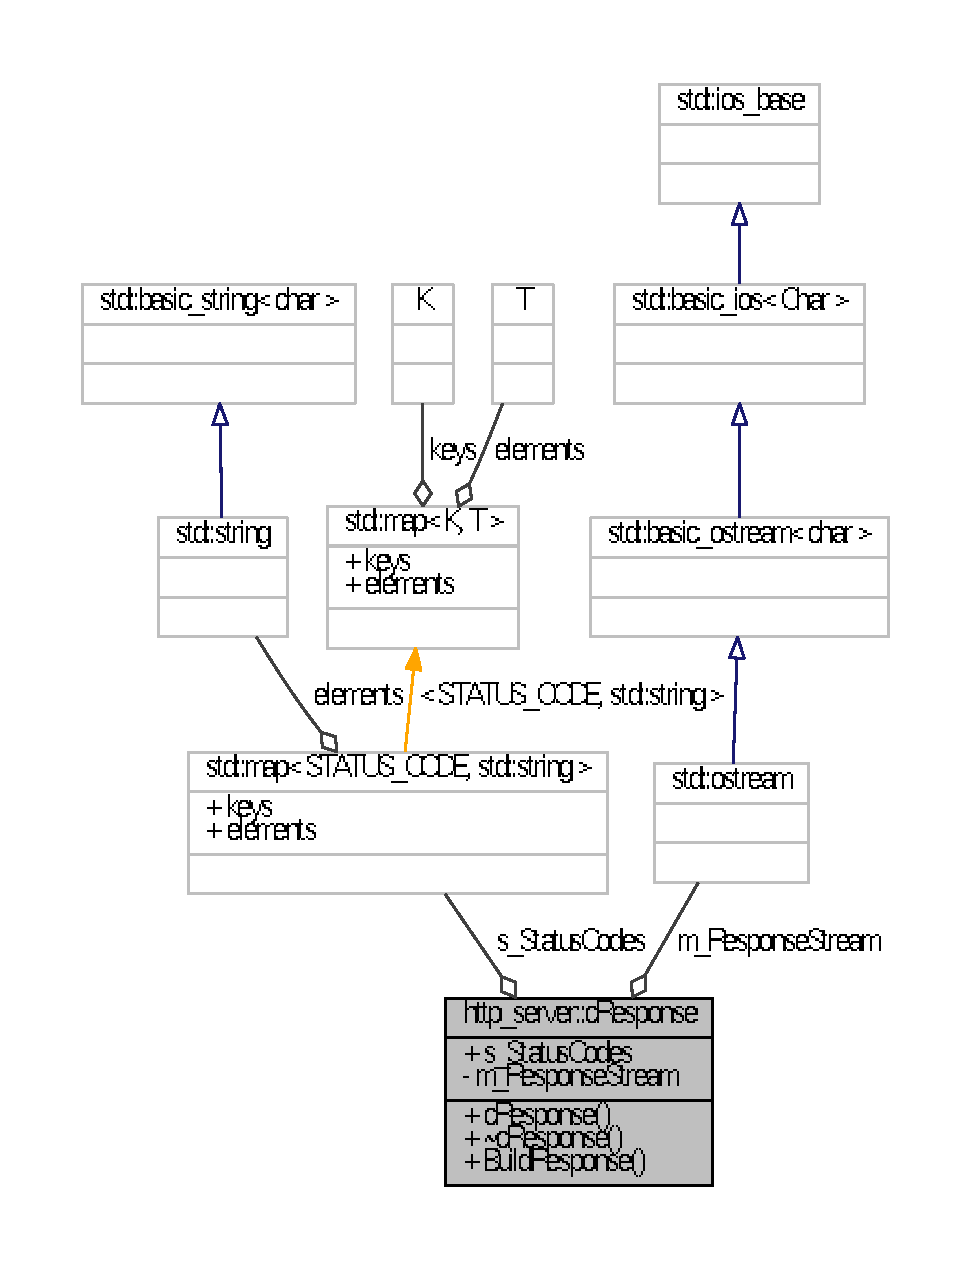
\includegraphics[width=350pt]{classhttp__server_1_1cResponse__coll__graph}
\end{center}
\end{figure}
\subsection*{\-Public \-Member \-Functions}
\begin{DoxyCompactItemize}
\item 
\hypertarget{classhttp__server_1_1cResponse_abdb27671f4818f6e6bcbc11530d18ebc}{{\bfseries c\-Response} (boost\-::asio\-::streambuf \&buffer)}\label{classhttp__server_1_1cResponse_abdb27671f4818f6e6bcbc11530d18ebc}

\item 
\hypertarget{classhttp__server_1_1cResponse_a484e013d4e453a86156b35adaf3eda5b}{void {\bfseries \-Build\-Response} (\-S\-T\-A\-T\-U\-S\-\_\-\-C\-O\-D\-E status\-\_\-code, const std\-::string \&resource\-\_\-body)}\label{classhttp__server_1_1cResponse_a484e013d4e453a86156b35adaf3eda5b}

\end{DoxyCompactItemize}
\subsection*{\-Static \-Public \-Attributes}
\begin{DoxyCompactItemize}
\item 
static std\-::map$<$ \-S\-T\-A\-T\-U\-S\-\_\-\-C\-O\-D\-E, \*
std\-::string $>$ {\bfseries s\-\_\-\-Status\-Codes}
\end{DoxyCompactItemize}
\subsection*{\-Private \-Attributes}
\begin{DoxyCompactItemize}
\item 
\hypertarget{classhttp__server_1_1cResponse_a26980e4d210c8f2e766d3ae987262160}{std\-::ostream {\bfseries m\-\_\-\-Response\-Stream}}\label{classhttp__server_1_1cResponse_a26980e4d210c8f2e766d3ae987262160}

\end{DoxyCompactItemize}


\subsection{\-Member \-Data \-Documentation}
\hypertarget{classhttp__server_1_1cResponse_a173245993bbac50f72d5a8528526cc26}{\index{http\-\_\-server\-::c\-Response@{http\-\_\-server\-::c\-Response}!s\-\_\-\-Status\-Codes@{s\-\_\-\-Status\-Codes}}
\index{s\-\_\-\-Status\-Codes@{s\-\_\-\-Status\-Codes}!http_server::cResponse@{http\-\_\-server\-::c\-Response}}
\subsubsection[{s\-\_\-\-Status\-Codes}]{\setlength{\rightskip}{0pt plus 5cm}std\-::map$<$ \-S\-T\-A\-T\-U\-S\-\_\-\-C\-O\-D\-E, std\-::string $>$ http\-\_\-server\-::c\-Response\-::s\-\_\-\-Status\-Codes\hspace{0.3cm}{\ttfamily  \mbox{[}static\mbox{]}}}}\label{classhttp__server_1_1cResponse_a173245993bbac50f72d5a8528526cc26}
{\bfseries \-Initial value\-:}
\begin{DoxyCode}
 boost::assign::map_list_of
        (OK,"200 OK")
        (ACCEPTED, "202 Accepted")
        (BAD_REQUEST, "400 Bad Request")
        (NOT_FOUND, "404 Not Found")
        (NOT_IMPLEMENTED, "501 Not Implemented")
\end{DoxyCode}


\-The documentation for this class was generated from the following files\-:\begin{DoxyCompactItemize}
\item 
http\-\_\-response.\-h\item 
http\-\_\-response.\-cpp\end{DoxyCompactItemize}

\hypertarget{structhttp__server_1_1method__}{
\section{http\-\_\-server\-:\-:method\-\_\- \-Struct \-Reference}
\label{structhttp__server_1_1method__}\index{http\-\_\-server\-::method\-\_\-@{http\-\_\-server\-::method\-\_\-}}
}


\-The documentation for this struct was generated from the following file\-:\begin{DoxyCompactItemize}
\item 
http\-\_\-request.\-cpp\end{DoxyCompactItemize}

%--- End generated contents ---

% Index
\newpage
\phantomsection
\addcontentsline{toc}{chapter}{Index}
\printindex

\end{document}
